\documentclass[
  shownotes,
  xcolor={svgnames},
  hyperref={colorlinks,citecolor=DarkBlue,linkcolor=DarkRed,urlcolor=DarkBlue}
  , aspectratio=169]{beamer}
\usepackage{animate}
\usepackage{amsmath}
\usepackage{amsfonts}
\usepackage{amssymb}
\usepackage{pifont}
\usepackage{mathpazo}
%\usepackage{xcolor}
\usepackage{multimedia}
\usepackage{fancybox}
\usepackage[para]{threeparttable}
\usepackage{multirow}
\setcounter{MaxMatrixCols}{30}
\usepackage{subcaption}
\usepackage{graphicx}
\usepackage{lscape}
\usepackage[compatibility=false,font=small]{caption}
\usepackage{booktabs}
\usepackage{ragged2e}
\usepackage{chronosys}
\usepackage{appendixnumberbeamer}
\usepackage{animate}
\setbeamertemplate{caption}[numbered]
\usepackage{color}
%\usepackage{times}
\usepackage{tikz}
\usepackage{comment} %to comment
%% BibTeX settings
\usepackage{natbib}
\bibliographystyle{apalike}
\bibpunct{(}{)}{,}{a}{,}{,}
\setbeamertemplate{bibliography item}{[\theenumiv]}

% Defines columns for bespoke tables
\usepackage{array}
\newcolumntype{L}[1]{>{\raggedright\let\newline\\\arraybackslash\hspace{0pt}}m{#1}}
\newcolumntype{C}[1]{>{\centering\let\newline\\\arraybackslash\hspace{0pt}}m{#1}}
\newcolumntype{R}[1]{>{\raggedleft\let\newline\\\arraybackslash\hspace{0pt}}m{#1}}


\usepackage{xfrac}


\usepackage{multicol}
\setlength{\columnsep}{0.5cm}

% Theme and colors
\usetheme{Boadilla}

% I use steel blue and a custom color palette. This defines it.
\definecolor{andesred}{HTML}{af2433}

% Other options
\providecommand{\U}[1]{\protect\rule{.1in}{.1in}}
\usefonttheme{serif}
\setbeamertemplate{itemize items}[default]
\setbeamertemplate{enumerate items}[square]
\setbeamertemplate{section in toc}[circle]

\makeatletter

\definecolor{mybackground}{HTML}{82CAFA}
\definecolor{myforeground}{HTML}{0000A0}

\setbeamercolor{normal text}{fg=black,bg=white}
\setbeamercolor{alerted text}{fg=red}
\setbeamercolor{example text}{fg=black}

\setbeamercolor{background canvas}{fg=myforeground, bg=white}
\setbeamercolor{background}{fg=myforeground, bg=mybackground}

\setbeamercolor{palette primary}{fg=black, bg=gray!30!white}
\setbeamercolor{palette secondary}{fg=black, bg=gray!20!white}
\setbeamercolor{palette tertiary}{fg=white, bg=andesred}

\setbeamercolor{frametitle}{fg=andesred}
\setbeamercolor{title}{fg=andesred}
\setbeamercolor{block title}{fg=andesred}
\setbeamercolor{itemize item}{fg=andesred}
\setbeamercolor{itemize subitem}{fg=andesred}
\setbeamercolor{itemize subsubitem}{fg=andesred}
\setbeamercolor{enumerate item}{fg=andesred}
\setbeamercolor{item projected}{bg=gray!30!white,fg=andesred}
\setbeamercolor{enumerate subitem}{fg=andesred}
\setbeamercolor{section number projected}{bg=gray!30!white,fg=andesred}
\setbeamercolor{section in toc}{fg=andesred}
\setbeamercolor{caption name}{fg=andesred}
\setbeamercolor{button}{bg=gray!30!white,fg=andesred}


\usepackage{fancyvrb}
\newcommand{\VerbBar}{|}
\newcommand{\VERB}{\Verb[commandchars=\\\{\}]}
\DefineVerbatimEnvironment{Highlighting}{Verbatim}{commandchars=\\\{\}}
% Add ',fontsize=\small' for more characters per line
\usepackage{framed}
\definecolor{shadecolor}{RGB}{248,248,248}
\newenvironment{Shaded}{\begin{snugshade}}{\end{snugshade}}
\newcommand{\AlertTok}[1]{\textcolor[rgb]{0.94,0.16,0.16}{#1}}
\newcommand{\AnnotationTok}[1]{\textcolor[rgb]{0.56,0.35,0.01}{\textbf{\textit{#1}}}}
\newcommand{\AttributeTok}[1]{\textcolor[rgb]{0.77,0.63,0.00}{#1}}
\newcommand{\BaseNTok}[1]{\textcolor[rgb]{0.00,0.00,0.81}{#1}}
\newcommand{\BuiltInTok}[1]{#1}
\newcommand{\CharTok}[1]{\textcolor[rgb]{0.31,0.60,0.02}{#1}}
\newcommand{\CommentTok}[1]{\textcolor[rgb]{0.56,0.35,0.01}{\textit{#1}}}
\newcommand{\CommentVarTok}[1]{\textcolor[rgb]{0.56,0.35,0.01}{\textbf{\textit{#1}}}}
\newcommand{\ConstantTok}[1]{\textcolor[rgb]{0.00,0.00,0.00}{#1}}
\newcommand{\ControlFlowTok}[1]{\textcolor[rgb]{0.13,0.29,0.53}{\textbf{#1}}}
\newcommand{\DataTypeTok}[1]{\textcolor[rgb]{0.13,0.29,0.53}{#1}}
\newcommand{\DecValTok}[1]{\textcolor[rgb]{0.00,0.00,0.81}{#1}}
\newcommand{\DocumentationTok}[1]{\textcolor[rgb]{0.56,0.35,0.01}{\textbf{\textit{#1}}}}
\newcommand{\ErrorTok}[1]{\textcolor[rgb]{0.64,0.00,0.00}{\textbf{#1}}}
\newcommand{\ExtensionTok}[1]{#1}
\newcommand{\FloatTok}[1]{\textcolor[rgb]{0.00,0.00,0.81}{#1}}
\newcommand{\FunctionTok}[1]{\textcolor[rgb]{0.00,0.00,0.00}{#1}}
\newcommand{\ImportTok}[1]{#1}
\newcommand{\InformationTok}[1]{\textcolor[rgb]{0.56,0.35,0.01}{\textbf{\textit{#1}}}}
\newcommand{\KeywordTok}[1]{\textcolor[rgb]{0.13,0.29,0.53}{\textbf{#1}}}
\newcommand{\NormalTok}[1]{#1}
\newcommand{\OperatorTok}[1]{\textcolor[rgb]{0.81,0.36,0.00}{\textbf{#1}}}
\newcommand{\OtherTok}[1]{\textcolor[rgb]{0.56,0.35,0.01}{#1}}
\newcommand{\PreprocessorTok}[1]{\textcolor[rgb]{0.56,0.35,0.01}{\textit{#1}}}
\newcommand{\RegionMarkerTok}[1]{#1}
\newcommand{\SpecialCharTok}[1]{\textcolor[rgb]{0.00,0.00,0.00}{#1}}
\newcommand{\SpecialStringTok}[1]{\textcolor[rgb]{0.31,0.60,0.02}{#1}}
\newcommand{\StringTok}[1]{\textcolor[rgb]{0.31,0.60,0.02}{#1}}
\newcommand{\VariableTok}[1]{\textcolor[rgb]{0.00,0.00,0.00}{#1}}
\newcommand{\VerbatimStringTok}[1]{\textcolor[rgb]{0.31,0.60,0.02}{#1}}
\newcommand{\WarningTok}[1]{\textcolor[rgb]{0.56,0.35,0.01}{\textbf{\textit{#1}}}}
\usepackage{graphicx}
\makeatletter


% colors
\definecolor{airforceblue}{rgb}{0.36, 0.54, 0.66}
\newcommand{\theme}{\color{andesred}}
\newcommand{\bk}{\color{black}}
\newcommand{\rd}{\color{red}}
\newcommand{\fg}{\color{ForestGreen}}
\newcommand{\bl}{\color{blue}}
\newcommand{\gr}{\color{black!60}}
\newcommand{\sg}{\color{DarkSlateGray}}
\newcommand{\br}{\color{SaddleBrown}}
\newcommand{\nv}{\color{Navy}}



% common math markups
\newcommand{\bs}[1]{\boldsymbol{#1}}
\newcommand{\mc}[1]{\mathcal{#1}}
\newcommand{\mr}[1]{\mathrm{#1}}
\newcommand{\bm}[1]{\mathbf{#1}}
\newcommand{\ds}[1]{\mathds{#1}}
\newcommand{\indep}{\perp\!\!\!\perp}

% shorthand
\newcommand{\sk}{\vspace{.5cm}}
\newcommand{\R}[1]{{\tt \nv #1}}
\newcommand{\til}{{\footnotesize$\bs{\stackrel{\sim}{}}$}}
\DeclareSymbolFont{extraup}{U}{zavm}{m}{n}
\DeclareMathSymbol{\vardiamond}{\mathalpha}{extraup}{87}

\usepackage{tikz}
% Tikz settings optimized for causal graphs.
\usetikzlibrary{shapes,decorations,arrows,calc,arrows.meta,fit,positioning}
\tikzset{
    -Latex,auto,node distance =1 cm and 1 cm,semithick,
    state/.style ={ellipse, draw, minimum width = 0.7 cm},
    point/.style = {circle, draw, inner sep=0.04cm,fill,node contents={}},
    bidirected/.style={Latex-Latex,dashed},
    el/.style = {inner sep=2pt, align=left, sloped}
}


\makeatother






%%%%%%%%%%%%%%% BEGINS DOCUMENT %%%%%%%%%%%%%%%%%%

\begin{document}

\title[Lecture 06]{Lecture 06: \\ Texto como Datos}
\subtitle{Aprendizaje y Minería de Datos para los Negocios}
\date{\today}

\author[Sarmiento-Barbieri]{Ignacio Sarmiento-Barbieri}
\institute[Uniandes]{Universidad de los Andes}


\begin{frame}[noframenumbering]
\maketitle
\end{frame}

%%%%%%%%%%%%%%%%%%%%%%%%%%%%%%%%%%%



%----------------------------------------------------------------------% 

\begin{frame}
\frametitle{Agenda}

\tableofcontents

\end{frame}

%----------------------------------------------------------------------%
\section{Text as Data}
%----------------------------------------------------------------------%
\begin{frame}[fragile]
\frametitle{Text as Data: Motivation}

{\bf We'll start with a story: \theme Slant in Partisan Speech}

  \begin{figure}[H] \centering
            \captionsetup{justification=centering}
              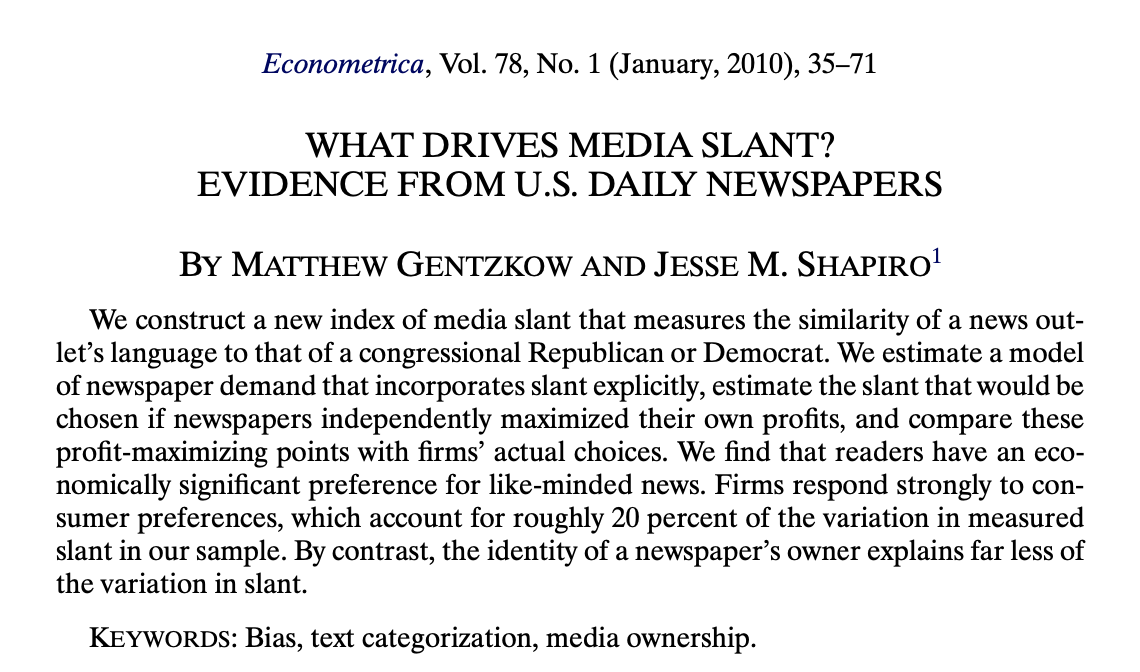
\includegraphics[scale=0.6]{figures/gentzgow_shapiro}
              
 \end{figure}

\end{frame}
%----------------------------------------------------------------------%
\begin{frame}[fragile]
\frametitle{Text as Data: Motivation}
\framesubtitle{Gentzkow and Shapiro: What drives media slant?  Evidence from
U.S. daily newspapers ({\it Econometrica}, 2010)}

\begin{itemize}
\item Build an economic model for newspaper demand that incorporates political partisanship (\rd Republican \bk vs \bl Democrat\bk)


 
\begin{itemize}
\item What would be independent profit-maximizing ``slant''?
\item Compare this to slant estimated from newspaper text.
\end{itemize}
\end{itemize}

\begin{center}
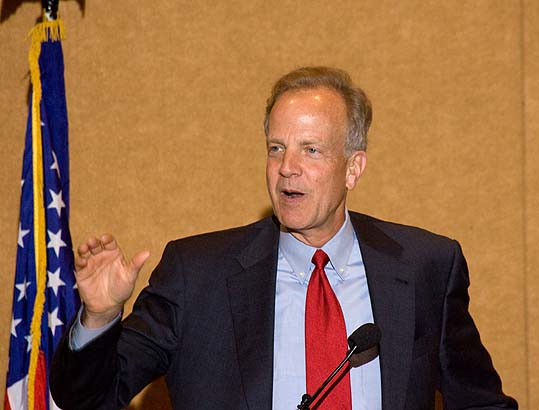
\includegraphics[width=1.7in]{figures/moran}
~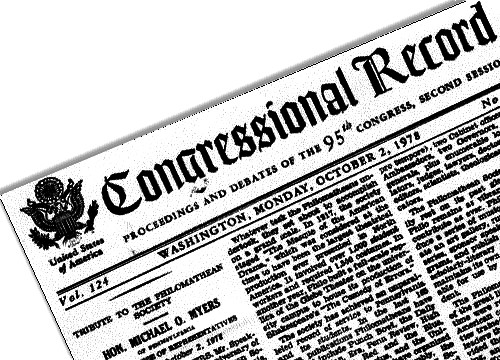
\includegraphics[width=1.75in]{figures/record}
\end{center}


 \end{frame}
%----------------------------------------------------------------------%
\begin{frame}[fragile]
\frametitle{Text as Data: Motivation}

\begin{itemize} 
\item Jerry Moran, R-KS, says ``death tax'' relatively often and his district
(Kansas 1st) voted 73\% for George W. Bush in 2004.
\end{itemize}

\begin{center}
$\bm{X_\text{text}} = f( \text{ideology}) \approx g(Y_{Bush})$

\vskip .25cm
$\bm{\Rightarrow}$ ``death tax'' is republican

\vskip .25cm
$\Rightarrow $ \theme the Wall Street Journal is slanted right.

\begin{itemize} 
\item William Jefferson, D-LA, says ``estate tax'' relatively often and his district
voted 24\% for George W. Bush in 2004.
\end{itemize}
\end{center}


\end{frame}
%----------------------------------------------------------------------%
\begin{frame}[fragile]
\frametitle{Text as Data: What is slant?}

\begin{itemize}
\item { Text:}  phrase-counts by speaker in 109$^{th}$ US Congress
(05-06)
\medskip
\item  { Sentiment:} two-party constituent vote-share for Bush in 2004.
\medskip

\item  Use covariance between  phrase frequencies ($f_{ij}$) and `Bush' sentiment ($y_i$)  to build an index of partisanship for text. 
\begin{center}\large
$z^{slant}_i= \sum_j \mr{cov}(f_j, y) f_{ij}$
\end{center}
\medskip
 \item For example, if phrase $j$ forms  a high proportion of what you say, and usage of phrase
 \medskip
\item $j$ is correlated with Bush vote-share, then this contributes a positive amount to your slant score.
\medskip
\vskip .2cm
\item  This is a type of {\it marginal regression}.
\end{itemize}
\end{frame}
%----------------------------------------------------------------------%
\begin{frame}[fragile]
\frametitle{Text as Data: Wordle} 


  \begin{figure}[H] \centering
            \captionsetup{justification=centering}
              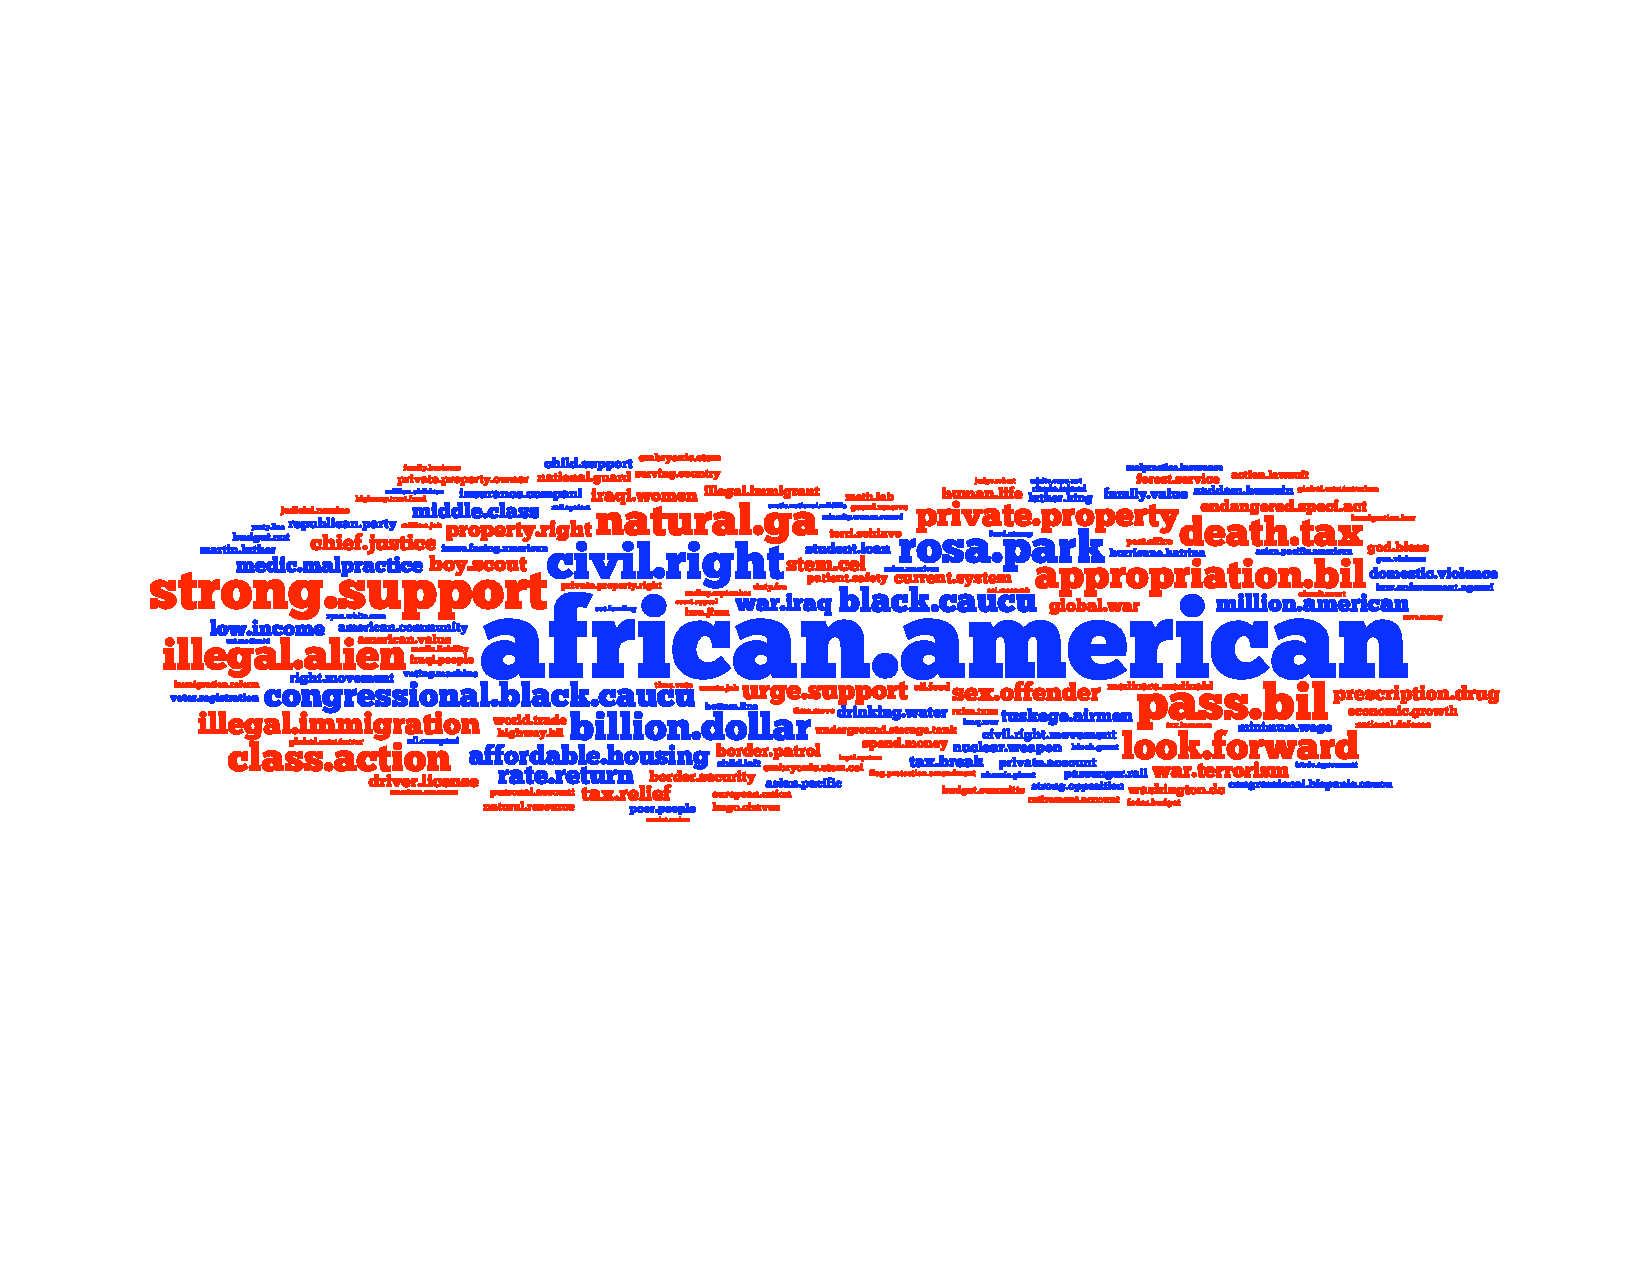
\includegraphics[width=4.5in]{figures/slantWrdl}
              
 \end{figure}

\begin{itemize}


\vskip .2cm
\item Colored by sign (\rd positive\bk, \bl negative\bk) \\ Size proportional to loading $\mr{cov}(f_j, y)$.\\

\vskip .2cm
\item Since $y$ is Republican vote-share, 
\begin{itemize}
\item Big positive is a right term and 
\item Big negative is a left term.
\end{itemize}
\end{itemize}

\end{frame}
%----------------------------------------------------------------------%

\begin{frame}

\begin{center}
{\bf Slant measure for speakers in the 109th Congress}
\vskip -.5cm
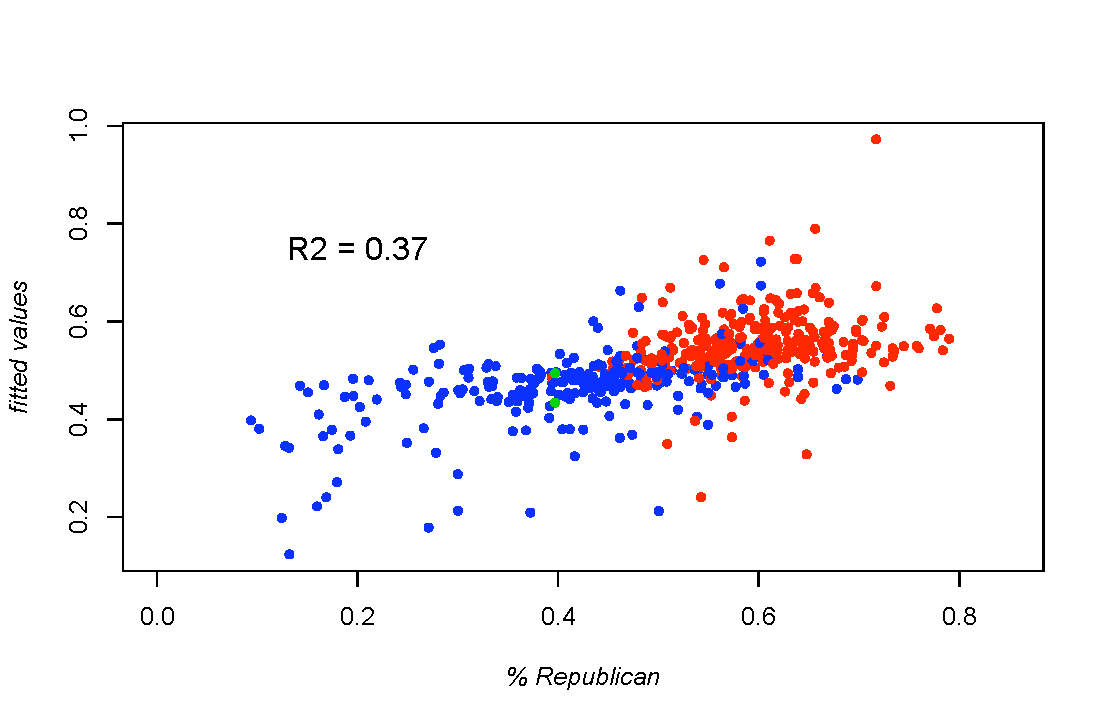
\includegraphics[width=4in]{figures/slant}\\
\end{center}

\vskip -.5cm
Democrats get low $z_\text{slant}$ and Republicans get high
$z_\text{slant}$.\\
\gr Do this for newspaper text and you'll get a similar picture

\end{frame}

%----------------------------------------------------------------------%
\begin{frame}[fragile]
\frametitle{Text as Data: The Big Picture}

\begin{itemize}


\item {\bf \theme Text is a vast source of data for business }
\medskip
\item It comes connected to interesting ``author'' variables 
\medskip
  \begin{itemize}
  \item What you buy, what you watch, your reviews
  \medskip
  \item Group membership, who you represent, who you email
  \medskip
  \item Market behavior, macro trends, the weather
  \end{itemize}

 
\item Opinion, subjectivity, etc.
\medskip
\item  Sentiment is {\it very} loosely defined:  Observables linked to the variables motivating language choice
\end{itemize}

\end{frame}

%----------------------------------------------------------------------%
\begin{frame}[fragile]
\frametitle{Text as Data: The Big Picture}

\begin{itemize}

\item {\bf \theme Text is also super high dimensional }

\medskip
\item And it gets higher dimensional as you observe more speech.


\medskip
\item Analysis of  phrase counts is the state of the art (hard to beat).


\item For example, occurrences by party for some partisan terms

\vskip .25cm
{\footnotesize
\begin{tabular}{|c|c|c|c|c|c|c}
Congress & State & Party & America & Death Tax & Estate Tax & $\cdots$
\\ \hline
\multirow{2}{*}{63} & \multirow{2}{*}{\sf NM} & {\sf dem}  & 108 &
  30 & 140 & \\ &
& {\sf gop}  & 100 &
  220 & 12  &
\end{tabular}}




\item Basic units of data

\begin{itemize}\bk
\item  doc-term count matrix $\bm{X}$ with rows $\bm{x}_i$.
\item  doc totals {\tt $\bm{m} = $ rowSums($\bm{X}$)} $=[m_1 \cdots m_n]$.
\item frequency matrix $\bm{F}=\bm{X}/\bm{m}$ with rows $\bm{f}_i$.
\end{itemize}

\end{itemize}

\end{frame}
%----------------------------------------------------------------------%
\section{Review
 \& Next Steps}
%----------------------------------------------------------------------%
\begin{frame}
\frametitle{Review \& Next Steps}
  
\begin{itemize} 
   \item XGBOOST
   \bigskip
   \item XGBOOST demo
   \bigskip
  \item Text as data
    \bigskip  
  \item  Next class:  More on text as data


\bigskip  
\item Questions? Questions about software? 

\end{itemize}
\end{frame}

%----------------------------------------------------------------------%
\section{Further Readings}
%----------------------------------------------------------------------%
\begin{frame}
\frametitle{Further Readings}

\begin{itemize}

  \item Chen, T., \& Guestrin, C. (2016, August). Xgboost: A scalable tree boosting system. In Proceedings of the 22nd acm sigkdd international conference on knowledge discovery and data mining (pp. 785-794).
  \medskip
  \item Chen, T., He, T., \& Benesty, M. (2018). XGBoost Documentation.
  \medskip
  \item Friedman, J., Hastie, T., \& Tibshirani, R. (2001). The elements of statistical learning (Vol. 1, No. 10). New York: Springer series in statistics.
  \medskip
  \item Taddy, M. (2019). Business data science: Combining machine learning and economics to optimize, automate, and accelerate business decisions. McGraw Hill Professional.

  
\end{itemize}

\end{frame}



%----------------------------------------------------------------------%
\subsection{Tokenization}
%----------------------------------------------------------------------%
\begin{frame}[fragile]
\frametitle{Information Retrieval and Tokenization}

\begin{itemize}


\item A passage in `{\it As You Like It}' from Shakepeare:

\medskip

~~~ {\sg All the world's a stage,\\
~~~ and all the men and women merely players:\\
~~~ they have their exits and their entrances;\\
~~~ and one man in his time plays many parts...}


\medskip
\item What the econometrian sees:

\medskip
\vspace{-.4cm}{\sg
\begin{verbatim}
   world stage men women play exit entrance time 
       1     1   2     1    2    1        1    1 
\end{verbatim}}

\medskip
\item This is the {\nv Bag-of-Words} representation of text.
\end{itemize}
\end{frame}


%----------------------------------------------------------------------%
\begin{frame}[fragile]
\frametitle{Possible tokenization steps} 

\begin{itemize}


\item Remove words that are super rare {\gr (in say $<\frac{1}{2}$\%, or $<15\%$ of docs; this is application specific)}.
 For example, if {\nv Argentine} occurs only once, it's useless for comparing documents.


\item Stemming:  `{\nv tax}' $\leftarrow$   taxing,  taxes, taxation, taxable, ... 

{\gr A stemmer cuts words to their root with a mix of rules and estimation.`Porter' is standard for English. }



\item  Remove a list of {\nv stop words} containing  irrelevant tokens.

{\gr ~~~~~If, and, but, who, what, the, they, their, a, or, ...}

{\nv Be careful: one person's stopword is another's key term.}


\item Convert to lowercase, drop numbers, punctuation, etc ...\\
{\gr Always application specific: e.g., don't drop {\tt :-)} from tweets.}
\end{itemize}


\end{frame}


%----------------------------------------------------------------------%
\begin{frame}[fragile]
\frametitle{The $n$-gram language model}

\begin{itemize}



\item An $n$-gram language model is one that describes a dialect through transition probabilities on $n$ consecutive words.

\medskip

\item An {\theme $n$-gram tokenization} counts length-$n$ sequences of words.\\
{\sg A unigram is a word, bigrams are transitions between words.}\\
{\gr e.g., {\tt world.stage}, {\tt stage.men}, {\tt men.women}, {\tt women.play}, ...}

\medskip

\item This can give you rich language data, but be careful: $n$-gram token vocabularies are very high dimensional ($p^n$)
\medskip
\item  More generally, you may have domain specific `clauses' that you wish to tokenize.
\medskip
\item  There is always a trade-off between complexity and generality. 
\medskip
\item {\theme Often best to just count words.}

\end{itemize}

\end{frame}
%----------------------------------------------------------------------%
\subsection{Tokenization Demo}
%----------------------------------------------------------------------%
\begin{frame}[fragile]
\frametitle{Tokenization Demo}

\begin{scriptsize}


\begin{Shaded}
\begin{Highlighting}[]
\CommentTok{\#\# the tm library (and related plugins) is R\textquotesingle{}s ecosystem for text mining.}
\CommentTok{\#\# for an intro see http://cran.r{-}project.org/web/packages/tm/vignettes/tm.pdf}
\KeywordTok{library}\NormalTok{(tm) }
\NormalTok{notes\textless{}{-}}\KeywordTok{readPDF}\NormalTok{(}\DataTypeTok{control =} \KeywordTok{list}\NormalTok{(}\DataTypeTok{text =} \StringTok{"{-}layout {-}enc UTF{-}8"}
  \NormalTok{))(}\DataTypeTok{elem=}\KeywordTok{list}\NormalTok{(}\DataTypeTok{uri=}\StringTok{"\textasciitilde{}/Papers/Beauty\_Hamermesh.pdf"}\NormalTok{), }\DataTypeTok{id=}\NormalTok{fname, }
  \DataTypeTok{language=}\StringTok{\textquotesingle{}en\textquotesingle{}}\NormalTok{)}
writeLines(content(notes)[1]) 
\end{Highlighting}
\end{Shaded}
\end{scriptsize}
\begin{tiny}



\begin{verbatim}
     ARTICLE IN PRESS
                                  Economics of Education Review 24 (2005) 369–376
                                                                                               www.elsevier.com/locate/econedurev
Beauty in the classroom: instructors’ pulchritude and putative
                                         pedagogical productivity
                                     Daniel S. Hamermesh, Amy Parker
                              Department of Economics, University of Texas, Austin, TX 78712-1173, USA
                                            Received 14 June 2004; accepted 21 July 2004
Abstract
   Adjusted for many other determinants, beauty affects earnings; but does it lead directly to the differences in
productivity that we believe generate earnings differences? We take a large sample of student instructional ratings for a
group of university teachers and acquire six independent measures of their beauty, and a number of other descriptors of
them and their classes. Instructors who are viewed as better looking receive higher instructional ratings, with the impact
of a move from the 10th to the 90th percentile of beauty being substantial. This impact exists within university
departments and even within particular courses, and is larger for male than for female instructors. Disentangling
whether this outcome represents productivity or discrimination is, as with the issue generally, probably impossible.
\end{verbatim}
\end{tiny}
\end{frame}
%----------------------------------------------------------------------%
\begin{frame}[fragile]
\frametitle{Tokenization Demo}

\begin{scriptsize}
\begin{Shaded}
\begin{Highlighting}[]
\KeywordTok{content}\NormalTok{(notes) \textless{}{-}}\KeywordTok{iconv}\NormalTok{(}\KeywordTok{content}\NormalTok{(notes), }\DataTypeTok{from=}\StringTok{"UTF{-}8"}\NormalTok{, }\DataTypeTok{to=}\StringTok{"ASCII"}\NormalTok{, }\DataTypeTok{sub=}\StringTok{""}\NormalTok{)}

\NormalTok{docs \textless{}{-}}\StringTok{ }\KeywordTok{Corpus}\NormalTok{(}\KeywordTok{VectorSource}\NormalTok{(notes))}

\KeywordTok{names}\NormalTok{(docs) \textless{}{-}}\StringTok{ }\KeywordTok{names}\NormalTok{(notes) }

\CommentTok{\#\# you can then do some cleaning here}
\CommentTok{\#\# tm\_map just maps some function to every document in the corpus}
\NormalTok{docs \textless{}{-}}\StringTok{ }\KeywordTok{tm\_map}\NormalTok{(docs, }\KeywordTok{content\_transformer}\NormalTok{(tolower)) }\CommentTok{\#\# make everything lowercase}
\NormalTok{docs \textless{}{-}}\StringTok{ }\KeywordTok{tm\_map}\NormalTok{(docs, }\KeywordTok{content\_transformer}\NormalTok{(removeNumbers)) }\CommentTok{\#\# remove numbers}
\NormalTok{docs \textless{}{-}}\StringTok{ }\KeywordTok{tm\_map}\NormalTok{(docs, }\KeywordTok{content\_transformer}\NormalTok{(removePunctuation)) }\CommentTok{\#\# remove punctuation}
\CommentTok{\#\# remove stopword. } 
\CommentTok{\#\#be careful with this: one\textquotesingle{}s stopwords are anothers keywords.}
\CommentTok{\# you could also do stemming; I don\textquotesingle{}t bother here.}
\NormalTok{docs \textless{}{-}}\StringTok{ }\KeywordTok{tm\_map}\NormalTok{(docs, }\KeywordTok{content\_transformer}\NormalTok{(removeWords), }\KeywordTok{stopwords}\NormalTok{(}\StringTok{"SMART"}\NormalTok{))}

\NormalTok{docs \textless{}{-}}\StringTok{ }\KeywordTok{tm\_map}\NormalTok{(docs, }\KeywordTok{content\_transformer}\NormalTok{(stripWhitespace)) }\CommentTok{\#\# remove excess white{-}space}
\end{Highlighting}
\end{Shaded}


\end{scriptsize}

\end{frame}
%----------------------------------------------------------------------%
\begin{frame}[fragile]
\frametitle{Tokenization Demo}


\begin{scriptsize}

\begin{Shaded}
\begin{Highlighting}[]
\CommentTok{\#\# create a doc{-}term{-}matrix}
\NormalTok{dtm \textless{}{-}}\StringTok{ }\KeywordTok{DocumentTermMatrix}\NormalTok{(docs)}
\NormalTok{dtm }
\end{Highlighting}
\end{Shaded}


\end{scriptsize}
\begin{tiny}



\begin{verbatim}
## <<DocumentTermMatrix (documents: 8, terms: 913)>>
## Non-/sparse entries: 1555/5749
## Sparsity           : 79%
## Maximal term length: 30
## Weighting          : term frequency (tf)
\end{verbatim}

\end{tiny}
\begin{scriptsize}

\begin{Shaded}
\begin{Highlighting}[]
\NormalTok{dtm \textless{}{-}}\StringTok{ }\KeywordTok{removeSparseTerms}\NormalTok{(dtm, }\FloatTok{0.75}\NormalTok{)}
\NormalTok{dtm }
\end{Highlighting}
\end{Shaded}

\end{scriptsize}
\begin{tiny}
\begin{verbatim}
## <<DocumentTermMatrix (documents: 8, terms: 156)>>
## Non-/sparse entries: 650/598
## Sparsity           : 48%
## Maximal term length: 15
## Weighting          : term frequency (tf)
\end{verbatim}
\end{tiny}
\end{frame}
%----------------------------------------------------------------------%
\begin{frame}[fragile]
\frametitle{Tokenization Demo}

\begin{scriptsize}


\begin{Shaded}
\begin{Highlighting}[]
\CommentTok{\#\# You can inspect them:}
\KeywordTok{inspect}\NormalTok{(dtm[}\DecValTok{1}\OperatorTok{:}\DecValTok{5}\NormalTok{,}\DecValTok{1}\OperatorTok{:}\DecValTok{8}\NormalTok{])}
\end{Highlighting}
\end{Shaded}
\end{scriptsize}
\begin{tiny}

\begin{verbatim}
## <<DocumentTermMatrix (documents: 5, terms: 8)>>
## Non-/sparse entries: 26/14
## Sparsity           : 35%
## ...
## Docs academic article beauty becker behavior biddle class classes
##    1        1       1      9      1        1      2     1       1
##    2        2       1      7      0        1      0     5       5
##    3        0       1      6      0        0      0     0       1
\end{verbatim}

\end{tiny}

\begin{scriptsize}
\begin{Shaded}
\begin{Highlighting}[]
\CommentTok{\#\# find words with greater than a min count}
\KeywordTok{findFreqTerms}\NormalTok{(dtm,}\DecValTok{50}\NormalTok{)}
\end{Highlighting}
\end{Shaded}

\end{scriptsize}
\begin{tiny}

\begin{verbatim}
## [1] "beauty"  "ratings"
\end{verbatim}

\end{tiny}
\begin{scriptsize}


\begin{Shaded}
\begin{Highlighting}[]
\CommentTok{\#\# or grab words whose count correlates with given words}
\KeywordTok{findAssocs}\NormalTok{(dtm, }\StringTok{"beauty"}\NormalTok{, }\FloatTok{.7}\NormalTok{) }
\end{Highlighting}
\end{Shaded}
\end{scriptsize}
\begin{tiny}


\begin{verbatim}
## $beauty
##  equation    effect     basic  positive     table perceived   results potential 
##      0.86      0.83      0.79      0.77      0.77      0.77      0.73      0.72 
##   problem   effects   instruc 
##      0.72      0.71      0.70
\end{verbatim}
\end{tiny}

\end{frame}
%----------------------------------------------------------------------%
\section{Text Regression}
%----------------------------------------------------------------------%
\begin{frame}
\frametitle{Text Regression}

\begin{itemize}
\item Once you have text in a numeric format, we can use all the tools we learned so far

\medskip

\item For example: Classify emails into spam

\begin{align}
\mr{logit}\left[{\tt spam} \right] = \alpha + f \beta
\end{align}
\item where $f_i=\frac{x_i}{\sum_j x_{ij}}$ are the normalized text counts

\end{itemize}

\end{frame}

%----------------------------------------------------------------------%
\subsection{Text Regression: Example}
%----------------------------------------------------------------------%
\begin{frame}[fragile]
\frametitle{Text Regression: Example (Gentzkow and Shapiro)}
\begin{scriptsize}



\begin{Shaded}
\begin{Highlighting}[]
\CommentTok{\#load packages}
\KeywordTok{library}\NormalTok{(textir) }
\CommentTok{\#load data}
\KeywordTok{data}\NormalTok{(congress109)}
\NormalTok{congress109Counts[}\KeywordTok{c}\NormalTok{(}\StringTok{"Barack Obama"}\NormalTok{,}\StringTok{"John Boehner"}\NormalTok{),}\DecValTok{995}\OperatorTok{:}\DecValTok{998}\NormalTok{]}
\end{Highlighting}
\end{Shaded}

\end{scriptsize}
\begin{tiny}


\begin{verbatim}
## 2 x 4 sparse Matrix of class "dgCMatrix"
##              stem.cel natural.ga hurricane.katrina trade.agreement
## Barack Obama        .          1                20               7
## John Boehner        .          .                14               .
\end{verbatim}

\end{tiny}
\begin{scriptsize}


\begin{Shaded}
\begin{Highlighting}[]
\NormalTok{congress109Ideology[}\DecValTok{1}\OperatorTok{:}\DecValTok{4}\NormalTok{,}\DecValTok{1}\OperatorTok{:}\DecValTok{5}\NormalTok{]}
\end{Highlighting}
\end{Shaded}
\end{scriptsize}
\begin{tiny}


\begin{verbatim}
##                            name party state chamber  repshare
## Chris Cannon       Chris Cannon     R    UT       H 0.7900621
## Michael Conaway Michael Conaway     R    TX       H 0.7836028
## Spencer Bachus   Spencer Bachus     R    AL       H 0.7812933
## Mac Thornberry   Mac Thornberry     R    TX       H 0.7776520
\end{verbatim}
\end{tiny}
\end{frame}
%----------------------------------------------------------------------%
\begin{frame}[fragile]
\frametitle{Text Regression: Example (Gentzkow and Shapiro)}

\begin{scriptsize}


\begin{Shaded}
\begin{Highlighting}[]
\KeywordTok{require}\NormalTok{(}\StringTok{"wordcloud"}\NormalTok{)}
\KeywordTok{wordcloud}\NormalTok{(}\DataTypeTok{words =} \KeywordTok{colnames}\NormalTok{(congress109Counts), }
          \DataTypeTok{freq =} \KeywordTok{colSums}\NormalTok{(congress109Counts),}
          \DataTypeTok{min.freq =} \DecValTok{100}\NormalTok{,}
          \DataTypeTok{scale =} \KeywordTok{c}\NormalTok{(}\DecValTok{3}\NormalTok{, }\FloatTok{0.1}\NormalTok{), }\DataTypeTok{max.words=}\DecValTok{200}\NormalTok{, }
          \DataTypeTok{random.order=}\OtherTok{FALSE}\NormalTok{, }\DataTypeTok{rot.per=}\FloatTok{0.35}\NormalTok{, }
          \DataTypeTok{colors=}\KeywordTok{brewer.pal}\NormalTok{(}\DecValTok{8}\NormalTok{, }\StringTok{"Set1"}\NormalTok{))}
\end{Highlighting}
\end{Shaded}
\end{scriptsize}

  \begin{figure}[H] \centering
            \captionsetup{justification=centering}
              
\includegraphics[scale=0.5]{figures/unnamed-chunk-3-1.pdf}
              
 \end{figure}


\end{frame}
%----------------------------------------------------------------------%
\begin{frame}[fragile]
\frametitle{Text Regression: Wordle (Wordclouds)}


\begin{scriptsize}


\begin{Shaded}
\begin{Highlighting}[]
\KeywordTok{tail}\NormalTok{(}\KeywordTok{colSums}\NormalTok{(congress109Counts))}
\end{Highlighting}
\end{Shaded}
\end{scriptsize}
\begin{tiny}



\begin{verbatim}
##          stem.cel        natural.ga hurricane.katrina   trade.agreement 
##              1699              1792              2020              2329 
## appropriation.bil   american.people 
##              2357              6256
\end{verbatim}
\end{tiny}

\begin{scriptsize}



\begin{Shaded}
\begin{Highlighting}[]
\KeywordTok{wordcloud}\NormalTok{(}\DataTypeTok{words =} \KeywordTok{colnames}\NormalTok{(congress109Counts), }
          \DataTypeTok{freq =} \KeywordTok{colSums}\NormalTok{(congress109Counts),}
          \DataTypeTok{min.freq =} \DecValTok{1000}\NormalTok{, }
          \DataTypeTok{scale =} \KeywordTok{c}\NormalTok{(}\DecValTok{3}\NormalTok{, }\FloatTok{0.1}\NormalTok{), }\DataTypeTok{max.words=}\DecValTok{30}\NormalTok{, }
          \DataTypeTok{random.order=}\OtherTok{FALSE}\NormalTok{, }\DataTypeTok{rot.per=}\FloatTok{0.35}\NormalTok{, }
          \DataTypeTok{colors=}\KeywordTok{brewer.pal}\NormalTok{(}\DecValTok{8}\NormalTok{, }\StringTok{"Set1"}\NormalTok{))}
\end{Highlighting}
\end{Shaded}

\end{scriptsize}


  \begin{figure}[H] \centering
            \captionsetup{justification=centering}
              
\includegraphics[scale=0.5]{figures/unnamed-chunk-5-1.pdf}
              
 \end{figure}



\end{frame}
%----------------------------------------------------------------------%
\begin{frame}[fragile]
\frametitle{Text Regression}

\begin{itemize}
  \item We can use {\tt LASSO}
\end{itemize}
\begin{scriptsize}

\begin{Shaded}
\begin{Highlighting}[]
\NormalTok{f \textless{}{-}}\StringTok{ }\NormalTok{congress109Counts}
\NormalTok{y \textless{}{-}}\StringTok{ }\NormalTok{congress109Ideology}\OperatorTok{$}\NormalTok{repshare}
\CommentTok{\# lasso }
\NormalTok{lassoslant \textless{}{-}}\StringTok{ }\KeywordTok{cv.gamlr}\NormalTok{(congress109Counts}\OperatorTok{\textgreater{}}\DecValTok{0}\NormalTok{, y)}
\NormalTok{B \textless{}{-}}\StringTok{ }\KeywordTok{coef}\NormalTok{(lassoslant}\OperatorTok{$}\NormalTok{gamlr)[}\OperatorTok{{-}}\DecValTok{1}\NormalTok{,]}
\KeywordTok{head}\NormalTok{(}\KeywordTok{sort}\NormalTok{(}\KeywordTok{round}\NormalTok{(B[B}\OperatorTok{!=}\DecValTok{0}\NormalTok{],}\DecValTok{4}\NormalTok{)),}\DecValTok{10}\NormalTok{)}
\end{Highlighting}
\end{Shaded}

\end{scriptsize}
\begin{tiny}


\begin{verbatim}
##    congressional.black.caucu                 family.value 
##                      -0.0839                      -0.0443 
##        issue.facing.american           voter.registration 
##                      -0.0324                      -0.0298 
##      minority.owned.business            strong.opposition 
##                      -0.0284                      -0.0264 
##                  civil.right        universal.health.care 
##                      -0.0259                      -0.0254 
## congressional.hispanic.caucu          ohio.electoral.vote 
##                      -0.0187                      -0.0183
\end{verbatim}
\end{tiny}

\end{frame}
%----------------------------------------------------------------------%
\begin{frame}[fragile]
\frametitle{Text Regression}

\begin{scriptsize}

\begin{Shaded}
\begin{Highlighting}[]
\KeywordTok{tail}\NormalTok{(}\KeywordTok{sort}\NormalTok{(}\KeywordTok{round}\NormalTok{(B[B}\OperatorTok{!=}\DecValTok{0}\NormalTok{],}\DecValTok{4}\NormalTok{)),}\DecValTok{10}\NormalTok{)}
\end{Highlighting}
\end{Shaded}

\end{scriptsize}
\begin{tiny}

\begin{verbatim}
##         illegal.alien        percent.growth   illegal.immigration 
##                0.0079                0.0083                0.0087 
##            global.war          look.forward            war.terror 
##                0.0098                0.0099                0.0114 
##      private.property        action.lawsuit          human.embryo 
##                0.0133                0.0142                0.0226 
## million.illegal.alien 
##                0.0328
\end{verbatim}


\end{tiny}

\end{frame}
%----------------------------------------------------------------------%
\section{Topic Models}
%----------------------------------------------------------------------%
\begin{frame}
\frametitle{Topic Models}

\begin{itemize}
\item Text is super high dimensional
\medskip
\item there is often abundant {\it unlabeled} text
\medskip
\item Some times unsupervized factor model is a popular and useful strategy with text data
\medskip
\item You can first fit a factor model to a giant corpus and use these factors for supervised learning on a subset of labeled documents.
\medskip
\item The unsupervised dimension reduction facilitates the supervised learning
\end{itemize}
\end{frame}
%----------------------------------------------------------------------%
\begin{frame}
\frametitle{Topic Models: Example}

\begin{itemize}


\item We have 6166 reviews, with an average length of 90 words per review, \url{we8there.com}. 
\medskip
\item A useful feature of these reviews is that they contain both text and a multidimensional rating on overall experience, atmosphere, food, service, and value. 
\medskip
\item For example, one user submitted a glowing review for Waffle House \#1258 in Bossier City, Louisiana: 
\medskip
{\tt \it 
I normally would not revue a Waffle House but this one deserves it. The workers, Amanda, Amy, Cherry, James and J.D. were the most pleasant crew I have seen. While it was only lunch, B.L.T. and chili, it was great. The best thing was the 50’ s rock and roll music, not to loud not to soft. This is a rare exception to what you all think a Waffle House is. Keep up the good work. \\
Overall: 5, Atmosphere: 5, Food: 5, Service: 5, Value: 5. 
}
\end{itemize}
\end{frame}
%----------------------------------------------------------------------%
\begin{frame}[fragile]
\frametitle{Topic Models: Example}
\begin{itemize}


\item After cleaning and Porter stemming, we are left with a vocabulary of 2640 bigrams. 
\item For example, the first review in the document-term matrix has nonzero counts on bigrams indicating a pleasant meal at a rib joint: 
\end{itemize}

\begin{scriptsize}

\begin{Shaded}
\begin{Highlighting}[]
\CommentTok{\#load packages}
\KeywordTok{library}\NormalTok{(textir) }
\CommentTok{\#load data}
\KeywordTok{data}\NormalTok{(we8there)}
\NormalTok{x \textless{}{-}}\StringTok{ }\NormalTok{we8thereCounts}
\NormalTok{x[}\DecValTok{1}\NormalTok{,x[}\DecValTok{1}\NormalTok{,]}\OperatorTok{!=}\DecValTok{0}\NormalTok{]}
\end{Highlighting}
\end{Shaded}

\end{scriptsize}
\begin{tiny}



\begin{verbatim}
## even though larg portion  mouth water     red sauc    babi back     back rib chocol mouss 
##           1            1            1            1            1            1            1 
## veri satisfi 
##            1 
\end{verbatim}
\end{tiny}
\end{frame}
%----------------------------------------------------------------------%
\begin{frame}[fragile]
\frametitle{Topic Models: Example}

\begin{itemize}


\item We can apply PCA to get a factor representation of the review text. 
\item  PC1 looks like it will be big and positive for positive reviews, 

\begin{scriptsize}

\begin{Shaded}
\begin{Highlighting}[]
\NormalTok{pca \textless{}{-}}\StringTok{ }\KeywordTok{prcomp}\NormalTok{(x, }\DataTypeTok{scale=}\OtherTok{TRUE}\NormalTok{) }\CommentTok{\# can take a long time}

\KeywordTok{tail}\NormalTok{(}\KeywordTok{sort}\NormalTok{(pca}\OperatorTok{$}\NormalTok{rotation[,}\DecValTok{1}\NormalTok{]))}
\end{Highlighting}
\end{Shaded}

\end{scriptsize}
\begin{tiny}

\begin{verbatim}
##     food great     staff veri     excel food high recommend     great food 
##    0.007386860    0.007593374    0.007629771    0.007821171    0.008503594 
##     food excel 
##    0.008736181
\end{verbatim}

\end{tiny}


\begin{scriptsize}

\item while PC4 will be big and negative 
\begin{Shaded}
\begin{Highlighting}[]
\KeywordTok{tail}\NormalTok{(}\KeywordTok{sort}\NormalTok{(pca}\OperatorTok{$}\NormalTok{rotation[,}\DecValTok{4}\NormalTok{]))}
\end{Highlighting}
\end{Shaded}
\end{scriptsize}
\begin{tiny}

\begin{verbatim}
##   order got after minut  never came   ask check readi order drink order 
##  0.05918712  0.05958572  0.06099509  0.06184512  0.06776281  0.07980788
\end{verbatim}
\end{tiny}




\end{itemize}
\end{frame}

%----------------------------------------------------------------------%
\subsection{PCA}
%----------------------------------------------------------------------%
\begin{frame}
\frametitle{Principal Component Analysis}

\begin{itemize}

  \item Dimensionality via main components

  \begin{align}
  X = (x_1 , x_2 , \dots , x_n )_{N \times K}
  \end{align}

  \item Factor: 

  \begin{align}
  F = X\delta \,\,\,\delta \in K
  \end{align}


  \item Idea: summarize the K variables in a single (F).
  \item Vocab: the coefficients of $\delta$ are the loadings: how much 'matters' each x s in the factor.
  \item Dimensionality: summarize the original K variables in a few $q <K$ factors.
  \end{itemize}

\end{frame}



%----------------------------------------------------------------------%
\begin{frame}
\frametitle{Algebra Review}

\begin{itemize}

\item Let $A_{m\times m}$. It exists 
\begin{itemize}
  \item a scalar $\lambda$ such that $Ax = \lambda x$ for a vector $x_{m\times 1}$, 
  \item if $x \neq 0$, then $\lambda$ is an eigenvalue of A. 
  \item and a vector $x$ is an eigenvector of A corresponding to the eigenvalue $\lambda$.
\end{itemize}

\item $A_{m\times m}$ with eigenvalues $\lambda_1, \lambda_2,\dots,\lambda_m$, then:

\begin{align}
tr(A) &= \sum_{i=1}^m \lambda_i \\
det(A) &= \Pi_{i=1}^m \lambda_i
\end{align}

\item If $A_{m\times m}$ has $m$ different eigenvalues, then the associated eigenvectors are all linearly independent.
\item Spectral decomposition: $A = P\Lambda P$, where $\Lambda = diag(\lambda_1, \dots \lambda_n )$ and $P$ is the matrix whose columns are the corresponding eigenvectors.
\end{itemize}

\end{frame}


%----------------------------------------------------------------------%
\begin{frame}
\frametitle{Factors via main components}

\begin{itemize}


\item $x_1, x_2, \dots, x_K$ , K vectors of N observations each.
\medskip
\item Factor: $F = X\delta$
\medskip
\item What is the 'best' linear combination of $x_1, x_2, \dots, x_K$ ?
\medskip
\item Best? Maximum variance. Why? The one that best reproduces variability original of all xs

\end{itemize}
\end{frame}
%----------------------------------------------------------------------%
\begin{frame}
\frametitle{Factors via main components}

\begin{itemize}
  \item Let
  \begin{itemize}
    \item $X = (x_1 , \dots , x_K)_{N \times K}$  , 
    \item $\Sigma V(X)$ 
    \item $\delta \in K$
 \end{itemize}
  \medskip
  \item $F = X\delta$ is a linear combination of $X$, with $V (X\delta) = \delta' \Sigma \delta$.
  \medskip
  \item Let's set up the problem as 
  \begin{align}
  \underset{\delta}{max}\,\,\, \delta' \Sigma \delta
  \end{align}
 \begin{itemize}
  \item It is obvious that the solution is to bring $\delta$ to infinity. 
 \end{itemize}
\end{itemize}
 \end{frame}
%----------------------------------------------------------------------%
\begin{frame}
\frametitle{Factors via main components}

\begin{itemize}
\item Let's "fix" the problem by normalizing $\delta$

\begin{align}
\underset{\delta}{max} \delta' \Sigma \delta \\ \nonumber
\text{subject to}  \\ \nonumber
\delta' \delta = 1 \nonumber
\end{align}
\item Let us call the solution to this problem $\delta^*$. 
\medskip
\item $F^* = X\delta^*$ is the 'best' linear combination of X. 

\end{itemize}
\end{frame}


%----------------------------------------------------------------------%
\begin{frame}
\frametitle{Factors via main components}

\begin{itemize}
\item Result: $\delta^*$ is the eigenvector corresponding to the largest eigenvalue of $\Sigma = V (X)$.
\medskip
\item $F^* = X\delta^*$ is the first principal component of $X$.
\medskip
\item Intuition: $X$ has $K$ columns and $Y = X\delta$ has only one. The factor built with the first principal component is the best way to represent the K variables of X using a single single variable.
\end{itemize}

\end{frame}

\begin{comment}
%----------------------------------------------------------------------%
\begin{frame}
\frametitle{Factors via main components}
Solution to the problem of the first principal component
Problem: max δ δ Σδ,
subject to δ δ = 1
Lagrange: L (δ, λ) = δ Σδ + λ (1 - δ δ). CPO:
Σ δ = λ δ
At the optimum, δ is the eigenvector corresponding to the eigenvalue λ of Σ. Premultiplying by δ and
remembering that δ δ = 1:
δ Σδ = λ
In order to maximize δ Σδ we must choose λ equal to the maximum eigenvalue of Σ and δ equal to
corresponding eigenvalue.
\end{frame}
%----------------------------------------------------------------------%
\begin{frame}
\frametitle{Factors via main components}
Factors such as unsupervised learning
Regression Y = Xβ + u. ˆY ≡ X
ˆ
β. Min ∑ (Y i - ˆY) 2
Learning is supervised: the discrepancy between Y and ˆY 'guides' learning.
The factor construction problem is unsupervised : we construct an index (the
factor) without ever seeing it.
We start with X N × K and end with F ∗
N × 1
= Xδ ∗
\end{frame}


\end{comment}


%----------------------------------------------------------------------%
\section{Topic Models}
%----------------------------------------------------------------------%
\begin{frame}
\frametitle{Topic Models}

\begin{itemize}
\item Text is super high dimensional
\medskip
\item Some times unsupervized factor model is a popular and useful strategy with text data
\medskip
\item You can first fit a factor model to a giant corpus and use these factors for supervised learning on a subset of labeled documents.
\medskip
\item The unsupervised dimension reduction facilitates the supervised learning
\end{itemize}
\end{frame}
%----------------------------------------------------------------------%
\begin{frame}
\frametitle{Topic Models: Example}

\begin{itemize}


\item We have 6166 reviews, with an average length of 90 words per review, \url{we8there.com}. 
\medskip
\item A useful feature of these reviews is that they contain both text and a multidimensional rating on overall experience, atmosphere, food, service, and value. 
\medskip
\item For example, one user submitted a glowing review for Waffle House \#1258 in Bossier City, Louisiana: 
\medskip
{\tt \it 
I normally would not revue a Waffle House but this one deserves it. The workers, Amanda, Amy, Cherry, James and J.D. were the most pleasant crew I have seen. While it was only lunch, B.L.T. and chili, it was great. The best thing was the 50’ s rock and roll music, not to loud not to soft. This is a rare exception to what you all think a Waffle House is. Keep up the good work. \\
Overall: 5, Atmosphere: 5, Food: 5, Service: 5, Value: 5. 
}
\end{itemize}
\end{frame}
%----------------------------------------------------------------------%
\begin{frame}[fragile]
\frametitle{Topic Models: Example}
\begin{itemize}


\item After cleaning and Porter stemming, we are left with a vocabulary of 2640 bigrams. 
\item For example, the first review in the document-term matrix has nonzero counts on bigrams indicating a pleasant meal at a rib joint: 
\end{itemize}

\begin{scriptsize}

\begin{Shaded}
\begin{Highlighting}[]
\CommentTok{\#load packages}
\KeywordTok{library}\NormalTok{(textir) }
\CommentTok{\#load data}
\KeywordTok{data}\NormalTok{(we8there)}
\NormalTok{x \textless{}{-}}\StringTok{ }\NormalTok{we8thereCounts}
\NormalTok{x[}\DecValTok{1}\NormalTok{,x[}\DecValTok{1}\NormalTok{,]}\OperatorTok{!=}\DecValTok{0}\NormalTok{]}
\end{Highlighting}
\end{Shaded}

\end{scriptsize}
\begin{tiny}



\begin{verbatim}
## even though larg portion  mouth water     red sauc    babi back     back rib chocol mouss 
##           1            1            1            1            1            1            1 
## veri satisfi 
##            1 
\end{verbatim}
\end{tiny}
\end{frame}
%----------------------------------------------------------------------%
\begin{frame}[fragile]
\frametitle{Topic Models: Example}

\begin{itemize}


\item We can apply PCA to get a factor representation of the review text. 
\item  PC1 looks like it will be big and positive for positive reviews, 

\begin{scriptsize}

\begin{Shaded}
\begin{Highlighting}[]
\NormalTok{pca \textless{}{-}}\StringTok{ }\KeywordTok{prcomp}\NormalTok{(x, }\DataTypeTok{scale=}\OtherTok{TRUE}\NormalTok{) }\CommentTok{\# can take a long time}

\KeywordTok{tail}\NormalTok{(}\KeywordTok{sort}\NormalTok{(pca}\OperatorTok{$}\NormalTok{rotation[,}\DecValTok{1}\NormalTok{]))}
\end{Highlighting}
\end{Shaded}

\end{scriptsize}
\begin{tiny}

\begin{verbatim}
##     food great     staff veri     excel food high recommend     great food 
##    0.007386860    0.007593374    0.007629771    0.007821171    0.008503594 
##     food excel 
##    0.008736181
\end{verbatim}

\end{tiny}


\begin{scriptsize}

\item while PC4 will be big and negative 
\begin{Shaded}
\begin{Highlighting}[]
\KeywordTok{tail}\NormalTok{(}\KeywordTok{sort}\NormalTok{(pca}\OperatorTok{$}\NormalTok{rotation[,}\DecValTok{4}\NormalTok{]))}
\end{Highlighting}
\end{Shaded}
\end{scriptsize}
\begin{tiny}

\begin{verbatim}
##   order got after minut  never came   ask check readi order drink order 
##  0.05918712  0.05958572  0.06099509  0.06184512  0.06776281  0.07980788
\end{verbatim}
\end{tiny}




\end{itemize}
\end{frame}

%----------------------------------------------------------------------%
\subsection{PCA}
\subsubsection{Theory}
%----------------------------------------------------------------------%
\begin{frame}
\frametitle{Principal Component Analysis}

\begin{itemize}

  \item Dimensionality via main components

  \begin{align}
  X = (x_1 , x_2 , \dots , x_K )_{N \times K}
  \end{align}

  \item Factor: 

  \begin{align}
  F = X\delta \,\,\,\delta \in K
  \end{align}


  \item Idea: summarize the K variables in a single (F).
  \item Vocab: the coefficients of $\delta$ are the loadings: how much 'matters' each x s in the factor.
  \item Dimensionality: summarize the original K variables in a few $q <K$ factors.
  \end{itemize}

\end{frame}



%----------------------------------------------------------------------%
\begin{frame}
\frametitle{Algebra Review}

\begin{itemize}

\item Let $A_{m\times m}$. It exists 
\begin{itemize}
  \item a scalar $\lambda$ such that $Ax = \lambda x$ for a vector $x_{m\times 1}$, 
  \item if $x \neq 0$, then $\lambda$ is an eigenvalue of A. 
  \item and a vector $x$ is an eigenvector of A corresponding to the eigenvalue $\lambda$.
\end{itemize}

\item $A_{m\times m}$ with eigenvalues $\lambda_1, \lambda_2,\dots,\lambda_m$, then:

\begin{align}
tr(A) &= \sum_{i=1}^m \lambda_i \\
det(A) &= \Pi_{i=1}^m \lambda_i
\end{align}

\item If $A_{m\times m}$ has $m$ different eigenvalues, then the associated eigenvectors are all linearly independent.
\item Spectral decomposition: $A = P\Lambda P$, where $\Lambda = diag(\lambda_1, \dots \lambda_n )$ and $P$ is the matrix whose columns are the corresponding eigenvectors.
\end{itemize}

\end{frame}


%----------------------------------------------------------------------%
\begin{frame}
\frametitle{Factors via main components}

\begin{itemize}


\item $x_1, x_2, \dots, x_K$ , K vectors of N observations each.
\medskip
\item Factor: $F = X\delta$
\medskip
\item What is the 'best' linear combination of $x_1, x_2, \dots, x_K$ ?
\medskip
\item Best? Maximum variance. Why? The one that best reproduces variability original of all xs

\end{itemize}
\end{frame}
%----------------------------------------------------------------------%
\begin{frame}
\frametitle{Factors via main components}

\begin{itemize}
  \item Let
  \begin{itemize}
    \item $X = (x_1 , \dots , x_K)_{N \times K}$  , 
    \item $\Sigma = V(X)$ 
    \item $\delta \in K$
 \end{itemize}
  \medskip
  \item $F = X\delta$ is a linear combination of $X$, with $V (X\delta) = \delta' \Sigma \delta$.
  \medskip
  \item Let's set up the problem as 
  \begin{align}
  \underset{\delta}{max}\,\,\, \delta' \Sigma \delta
  \end{align}
 \begin{itemize}
  \item It is obvious that the solution is to bring $\delta$ to infinity. 
 \end{itemize}
\end{itemize}
 \end{frame}
%----------------------------------------------------------------------%
\begin{frame}
\frametitle{Factors via main components}

\begin{itemize}
\item Let's "fix" the problem by normalizing $\delta$

\begin{align}
\underset{\delta}{max}\,\, \delta' \Sigma \delta \\ \nonumber
\text{subject to}  \\ \nonumber
\delta' \delta = 1 \nonumber
\end{align}
\item Let us call the solution to this problem $\delta^*$. 
\medskip
\item $F^* = X\delta^*$ is the 'best' linear combination of X. 
\medskip
\item Intuition: $X$ has $K$ columns and $Y = X\delta$ has only one. The factor built with the first principal component is the best way to represent the K variables of X using a single single variable.
\end{itemize}
\end{frame}



%----------------------------------------------------------------------%
\begin{frame}
\frametitle{Factors via main components}

\begin{itemize}


\item Solution to the problem of the first principal component
\item Problem: 
\begin{align}
\underset{\delta}{max}\,\, \delta' \Sigma \delta \,\, \text{  s.t.}  \,\, \delta' \delta = 1 \nonumber
\end{align}
\item Seting up the Lagrangian $$\mathcal{L}(\delta,\lambda) = \delta' \Sigma \delta + \lambda(1-\delta'\delta)$$

\item CPO

\begin{align}
\Sigma \delta = \lambda \delta
\end{align}

\item At the optimum, $\delta$ is the eigenvector corresponding to the eigenvalue $\lambda$ of $\Sigma$. 
\item Premultiplying by $\delta$ and  remembering that $\delta'\delta = 1$:
\begin{align}
\delta \Sigma \delta = \lambda
\end{align}
\footnotesize
\item In order to maximize $\delta \Sigma \delta $ we must choose $\lambda$ equal to the maximum eigenvalue of $\Sigma$ and $\delta$ is the corresponding eigenvalue.
\end{itemize}
\end{frame}


%----------------------------------------------------------------------%
\begin{frame}
\frametitle{Factors is unsupervised learning}

\begin{itemize}

\item Recall that 
\begin{itemize}
  \item In regression we had
  \begin{align}
  y =X \beta +u
  \end{align}
 \item We minimized the MSE
 \begin{align}
 min \sum (y_i-\hat{y})^2
 \end{align}

\item Learning is supervised: the difference between $y$ and $\hat y$ ``guides'' the learning.
\end{itemize}
\item  The factor construction problem is unsupervised: we construct an index (the factor) without ever seeing it.
\begin{itemize}
\item We start with 
\begin{align}
X_{n\times k}
\end{align}
\item We end  with 
\begin{align}
F^*_{n\times 1} = X\delta^*
\end{align}
\end{itemize}
\end{itemize}
\end{frame}



%----------------------------------------------------------------------%
\begin{frame}
\frametitle{q main components}

\begin{itemize}

\item The first main component? Are there others?

\item Let's consider the following problem:
\begin{align}
\underset{\delta_2}{max}\,\, \delta_2' \Sigma \delta_2 \\ \nonumber
\text{subject to}  \\ \nonumber
\delta_2' \delta_2 &= 1 \\ \nonumber
and \\ \nonumber
Cov(\delta'_2 X,\delta^{*'}X) &=0 \\ \nonumber
\end{align}

\item $F_2^*=X\delta^*_2$ is the second principal component : the best linear combination which is
orthogonal to the best initial linear combination.
\item Recursively, using this logic you can form q  main components. 
\item Note that algebraically we could construct $q = K$ factors.
\end{itemize}
\end{frame}

%----------------------------------------------------------------------%
\begin{frame}
\frametitle{q main components}

\begin{itemize}
\item Let $\lambda_1,\dots,\lambda_K$ be the eigenvalues of $\Sigma = V(X)$, ordered from highest to lowest, and $p_1 , \dots , p_K$ the corresponding eigenvectors. Let us call $P$ the matrix of eigenvectors.
\medskip
\item Result: $\delta_j = p_j$ , $\forall j$ ('loadings' of the principal components =ordered eigenvectors of $\Sigma$).
\medskip
\item Let $F_j = X \delta_j$ , $j = 1, \dots, K$ be the j-th principal component. It's easy to see that
\begin{align}
V (F_j ) = \delta'_j \Sigma \delta_j = p_j P\Lambda P p_j = \lambda_j
\end{align}

(the variance of the j-th principal component is the j-th ordered eigenvalue of $\Sigma$).
\end{itemize}


\end{frame}


%----------------------------------------------------------------------%
\begin{frame}
\frametitle{Relative importance of factors}
\begin{itemize}


\item The total variance of X is the sum of the variances of $x_j$ , $j = 1, ..., K$, that is $trace(\Sigma)$
\item It is easy to show that:
\begin{align}
trace(\Sigma) = trace(P \Lambda P')= trace(PP' \Lambda ) = \sum_{j=1}^K \lambda_j= \sum_{j=1}^K V(F_j)
\end{align}
\item Then

\begin{align}
\frac{\lambda_k}{\sum_{j=1}^K \lambda_j}
\end{align}

\item measures the relative importance of the jth principal component.
\end{itemize}
\end{frame}

%----------------------------------------------------------------------%
\begin{frame}
\frametitle{Selection of factors}

\begin{itemize}


\item Look at the importance of the first principal components. If the first one explains a lot, there is really only one dimension (one dimension explains almost everything).
\bigskip
\item The coefficients of the eigenvectors are weights. See how each of the variables 'contributes' in each factor.
\bigskip
\item Beware of differences in scale. Always standardize 
\end{itemize}
\end{frame}


%----------------------------------------------------------------------%
\begin{frame}
\frametitle{Selection of factors}

\begin{itemize}
\item Let the columns of X be standardized, so that each variable has unit variance. 
\item In this case:

\begin{align}
trace(\Sigma) =  \sum_{j=1}^K V(F_j) = K
\end{align}

\item and recall $\sum_{j=1}^K \lambda_j= \sum_{j=1}^K V(F_j)$ then

\begin{align}
 \sum_{j=1}^K \lambda_j = K
\end{align}

\item On average, each factor contributes one unit. When $\lambda_j>1$, that factor it explains the total variance more than the average. $\rightarrow$ Retain the factors with $\lambda_j > 1$ 

\end{itemize}


\end{frame}




%----------------------------------------------------------------------%
\subsubsection{Factor Computation}
%----------------------------------------------------------------------%
\begin{frame}[fragile]
\frametitle{Useful Tips: Factor Computation}


\begin{itemize}


\item As a practical aside, note that \texttt{prcomp} converts x here from sparse to dense matrix storage.

\item For really big text DTMs, which will be very sparse, this will cause you to run out of memory. 

\item A big data strategy for PCA is to first calculate the covariance matrix for x and then obtain PC rotations as the eigenvalues of this covariance matrix. 

\item The first step can be done using sparse matrix algebra. 

\item The rotations are then available as

\begin{verbatim}
## eigen( xvar, symmetric = TRUE)$vec. 
\end{verbatim}


\item There are also approximate PCA algorithms available for fast factorization on big data. See, for example, the \texttt{irlba} package for R. 
\end{itemize}
\end{frame}

%----------------------------------------------------------------------%
\subsubsection{Factor Interpretation}
%----------------------------------------------------------------------%
\begin{frame}
\frametitle{Factor Interpretation}

\begin{itemize}
\item $F_s = X\delta_s$ : 'loadings' often suggest that a factor works as a 'index' of a group of variables.
\bigskip
\item Idea: look at the 'loadings'
\bigskip
\item Caution: factors via principal components are orthogonal recursively.
\end{itemize}


\end{frame}


%----------------------------------------------------------------------%
\begin{frame}[fragile]
\frametitle{Factor Interpretation: Example}


\begin{itemize}
\item {\bf Congress and \theme Roll Call Voting}
\bigskip
\begin{itemize}
  \item Votes in which names and positions are recorded are called `roll calls'.
  \medskip
  \item The site {\tt voteview.com} archives vote records and the R package { \tt pscl} has tools for this data.
  \medskip
  \item 445 members in the last US House  (the $111^{th}$)
  \medskip
  \item 1647 votes:  \theme nea = -1, \nv yea=+1, \gr missing = 0.
  \medskip
  \item This leads to a large matrix of observations that can probably be reduced to simple factors {\gr (party)}.
\end{itemize}
\end{itemize}





\end{frame}


%----------------------------------------------------------------------%
\begin{frame}[fragile]
\frametitle{Factor Interpretation}

\begin{itemize}

  \item Vote components in the $\bs{111^{th}}$ house
 
 \item Each PC is $F_s = X\delta_s$ 

  \begin{figure}[H] \centering
            \captionsetup{justification=centering}
              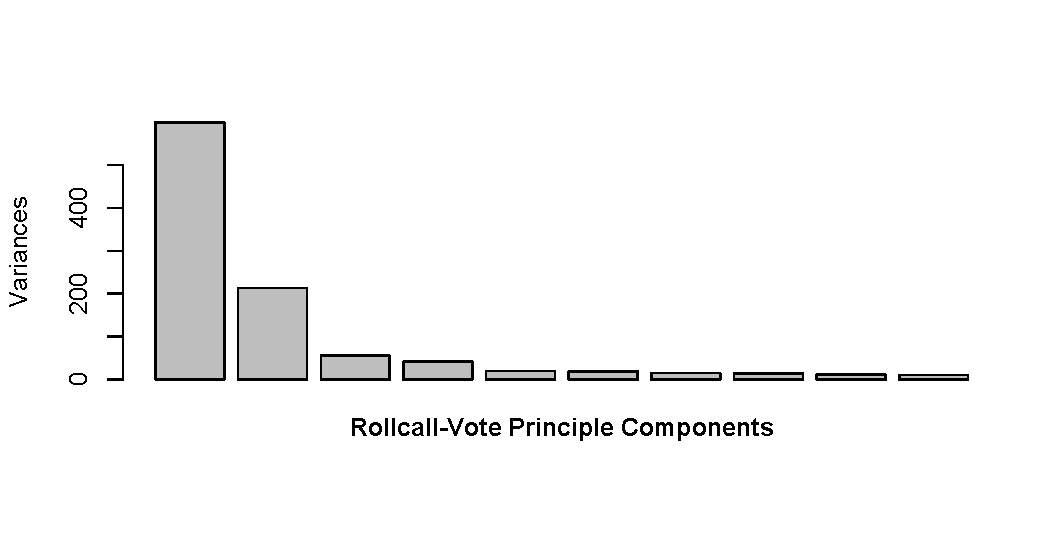
\includegraphics[scale=0.5]{figures/VOTEscree}
              
 \end{figure}

\item Huge drop in variance from $1^{st}$ to $2^{nd}$ and  $2^{nd}$ to $3^{rd}$ PC.
\item Poli-Sci holds that PC1 is usually enough to explain congress. \\\sg 2nd component has been important twice: 1860's and 1960's.

\end{itemize}


\end{frame}

%----------------------------------------------------------------------%
\begin{frame}[fragile]
\frametitle{Factor Interpretation}



\begin{itemize}

  \item Vote components in the $\bs{111^{th}}$ house
 
 \item Each PC is $F_s = X\delta_s$ 

  \begin{figure}[H] \centering
            \captionsetup{justification=centering}
              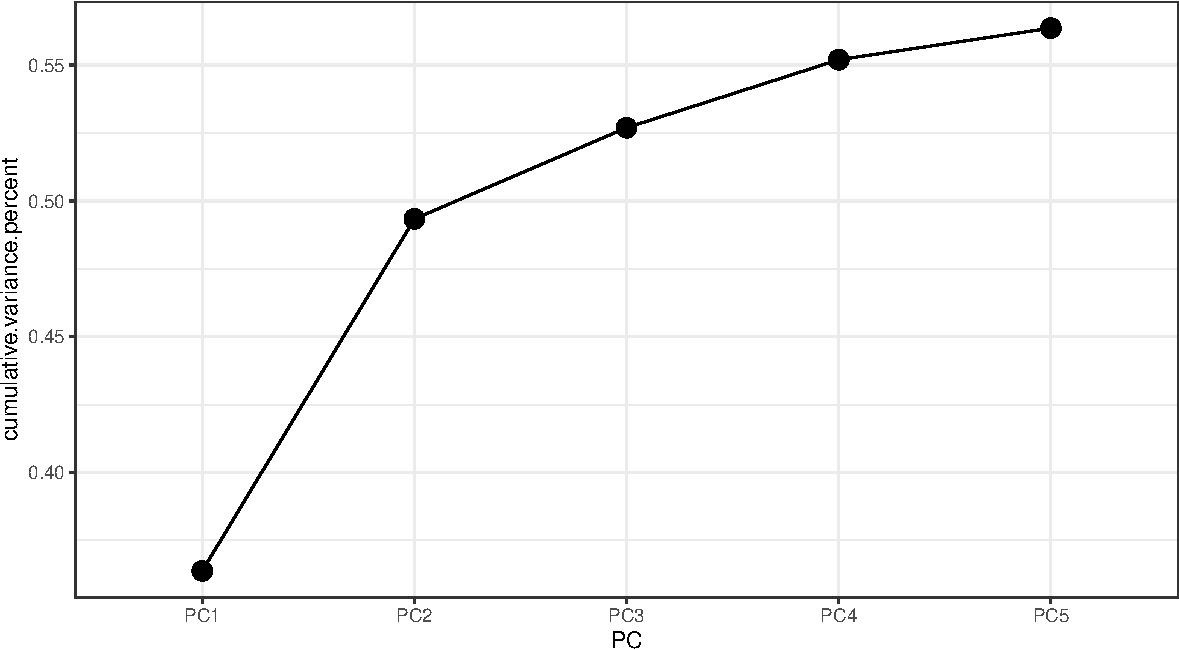
\includegraphics[scale=0.4]{figures/scree_plot}
              
 \end{figure}

\item Huge drop in variance from $1^{st}$ to $2^{nd}$ and  $2^{nd}$ to $3^{rd}$ PC.
\item Poli-Sci holds that PC1 is usually enough to explain congress. \\\sg 2nd component has been important twice: 1860's and 1960's.

\end{itemize}

\end{frame}

%----------------------------------------------------------------------%
\begin{frame}[fragile]
\frametitle{Factor Interpretation}

\begin{itemize}
\item Top two PC directions in the $\bs{111^{th}}$ house



  \begin{figure}[H] \centering
            \captionsetup{justification=centering}
              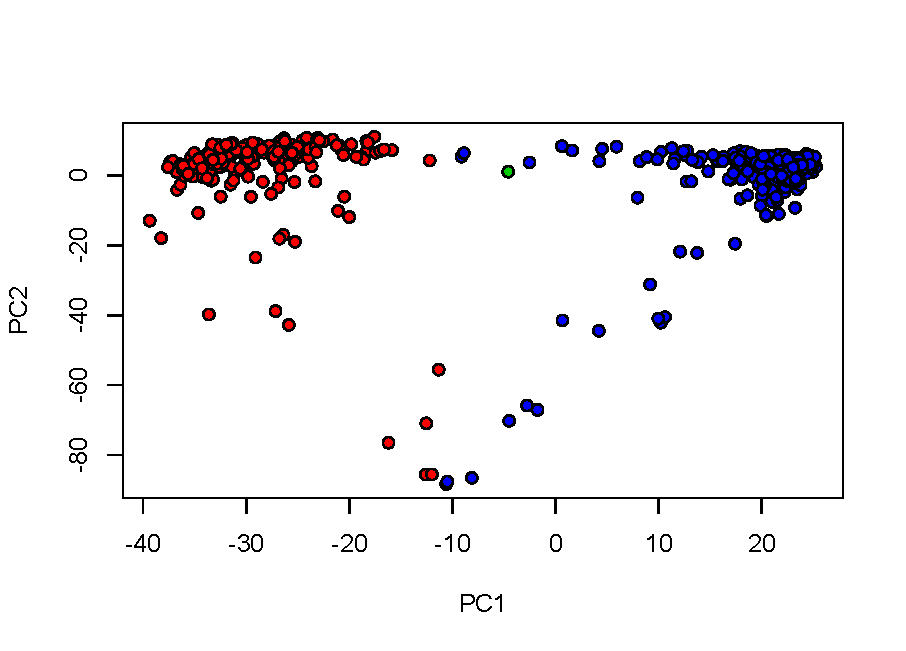
\includegraphics[scale=.5]{figures/VOTEpc}
 \end{figure}




  \item Republicans in red and Democrats in blue: 
  \begin{itemize}
  \item Clear separation on the first principal component.
  \item The second component looks orthogonal to party.
  \end{itemize}
\end{itemize}


\end{frame}


%----------------------------------------------------------------------%
\begin{frame}[fragile]
\frametitle{Factor Interpretation}




{\scriptsize \nv

{\theme \tt \#\# Far right (very conservative) \vspace{-.25cm}}
\begin{verbatim}
> sort(votepc[,1])
     BROUN (R GA-10)       FLAKE (R AZ-6)   HENSARLIN (R TX-5) 
         -39.3739409          -38.2506713          -37.5870597 
\end{verbatim}

{\theme \tt \#\# Far left (very liberal) \vspace{-.25cm}}
\begin{verbatim}
> sort(votepc[,1], decreasing=TRUE)
    EDWARDS (D MD-4)   PRICE (D NC-4)    MATSUI (D CA-5)      
         25.2915083        25.1591151         25.1248117     
\end{verbatim}       
  

{\theme \tt \#\# social issues? immigration? no clear pattern\vspace{-.25cm}}
\begin{verbatim}
> sort(votepc[,2])
     SOLIS (D CA-32) GILLIBRAND (D NY-20)      PELOSI (D CA-8) 
        -88.31350926         -87.58871687         -86.53585568 
   STUTZMAN (R IN-3)       REED (R NY-29)      GRAVES (R GA-9) 
        -85.59217310         -85.53636319         -76.49658108 
\end{verbatim}
}

\begin{itemize}
  \item PC1 is easy to read, PC2 is ambiguous (is it even meaningful?)
\end{itemize}


\end{frame}

%----------------------------------------------------------------------%
\begin{frame}[fragile]
\frametitle{Factor Interpretation}

\begin{itemize}
  \item {\bf \nv High PC1-loading votes are \theme  ideological battles.} 
  \item These tend to have  informative voting across party lines.


 \begin{figure}[H] \centering
            \captionsetup{justification=centering}
              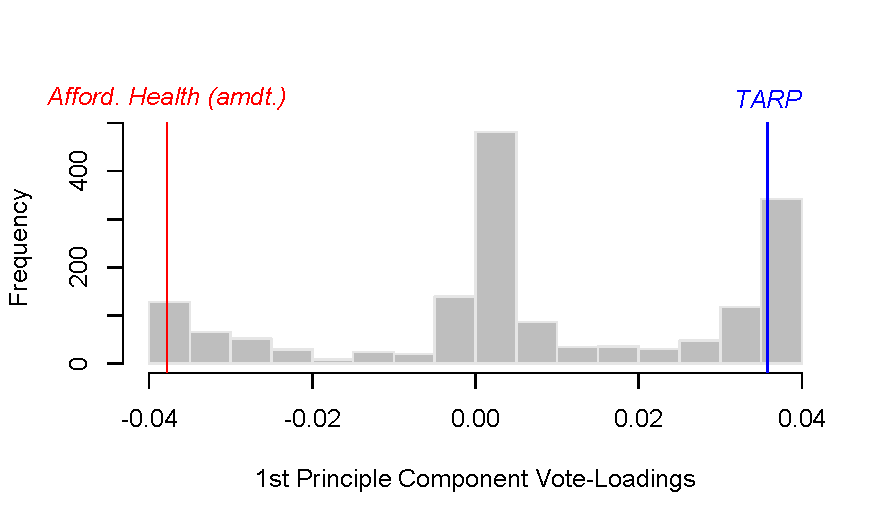
\includegraphics[scale=.5]{figures/VOTEloads}
 \end{figure}


 \footnotesize 
\item A vote for Repulican amendments to `Affordable Health Care for America' strongly indicates a negative PC1 (more conservative), while \\a vote for Troubled Asset Relief Program (TARP) indicates a positive PC1 (more progressive).
\end{itemize}

\end{frame}

%----------------------------------------------------------------------%
\begin{frame}[fragile]
\frametitle{Factor Interpretation}

\begin{itemize}
\item Look at the largest loadings in $\delta_{2}$ to discern an interpretation.



{\nv \scriptsize 
\begin{verbatim}
  > loadings[order(abs(loadings[,2]), decreasing=TRUE)[1:5],2]
   Vote.1146   Vote.658  Vote.1090  Vote.1104  Vote.1149 
  0.05605862 0.05461947 0.05300806 0.05168382 0.05155729 
\end{verbatim} }
  
\vskip -.25cm
\item These votes all correspond to near-unanimous  symbolic action.

\vskip .25cm
\bk
\item For example, 429 legislators voted for resolution 1146: \\
`{\sg Supporting the goals and ideals of a Cold War Veterans Day}'\\
{\gr If you didn't vote for this, you weren't in the house.}


 \item {{\theme Mystery Solved: } the second PC is just attendance!}
\vspace{- .1cm}
{\nv \scriptsize 
\begin{verbatim}
 > sort(rowSums(votes==0), decreasing=TRUE)
      SOLIS (D CA-32) GILLIBRAND (D NY-20)       REED (R NY-29) 
                 1628                 1619                 1562 
    STUTZMAN (R IN-3)      PELOSI (D CA-8)      GRAVES (R GA-9) 
                 1557                 1541                 1340 
\end{verbatim}}
\vspace{- .25cm}
\end{itemize}

\end{frame}
%----------------------------------------------------------------------%
\begin{frame}[fragile]
\frametitle{Principal Component Regression}


\begin{itemize}




\item The concept is very simple: instead of regressing onto $X$, use a lower dimension set of principal components $F$ as covariates.

\medskip
\item This works well for a few reasons:
\begin{itemize}
\item PCA reduces dimension, which is always good.
\item Higher variance covariates are good in regression, and we choose
  the top PCs to have highest variance.
\item The PCs are independent: no multicollinearity.
\end{itemize}


\item The 2-stage algorithm is straightforward. For example,

{\nv 
\begin{semiverbatim}\vspace{.25cm}\small
         mypca = prcomp(X, scale=TRUE)
         z = predict(mypca)[,1:K]
         reg = glm(y~., data=as.data.frame(z))
\end{semiverbatim}
}

\end{itemize}


\end{frame}

%----------------------------------------------------------------------%
\subsection{Latent Dirichlet Allocation}
%----------------------------------------------------------------------%
\begin{frame}
\frametitle{Latent Dirichlet Allocation}

\begin{itemize}


\item The approach of using PCA to factorize text was common before the 2000s. 
\medskip
\item Versions of this algorithm were referred to under the label latent semantic analysis. 
\medskip
\item However, this changed with the introduction of topic modeling, also known as Latent Dirichlet Allocation (LDA), by Blei et al. in 2003. 
\medskip
\item These authors pointed out that the squared error loss (i.e., Gaussian model) implied by PCA is inappropriate for analysis of sparse word-count data. 
\medskip
\item Instead, they proposed you take the bag-of-words representation seriously and model token counts as realizations from a multinomial distribution. 
\end{itemize}

\end{frame}


%----------------------------------------------------------------------%
\begin{frame}
\frametitle{Latent Dirichlet Allocation}

\begin{itemize}

\item That is, they proposed topic models as a multinomial factor model. 
\medskip
\item Topic models are built on a simple document generation process: 
\medskip
\begin{itemize}

\item  For each word, pick a “topic” k. This topic is defined through a probability vector over words, say, $\theta_k$ with probability $\theta_{kj}$ for each word j. 
\medskip
\item Then draw the word according to the probabilities encoded in $\theta_k$ . 
\medskip
\end{itemize}
\item After doing this over and over for each word in the document, you have proportion $\omega_{i1}$ from topic 1, $\omega_{i2}$ from topic 2, and so on. 

\end{itemize}
\end{frame}
%----------------------------------------------------------------------%
\begin{frame}
\frametitle{Latent Dirichlet Allocation}

\begin{itemize}


\item This basic generation process implies that the full vector of word counts, $x_i$, has a multinomial  distribution: 
\begin{align}
x_i \sim MN(\omega_{i1}\theta_1+\dots+\omega_{iK}\theta_K,m_i)
\end{align}
\item where $m_i=\sum_j x_{ij}$ is the total document length and, for example, 
\item the probability of word j in document i will be $\sum_k \omega_{ik}\theta_{kj}$

\end{itemize}


\end{frame}
%----------------------------------------------------------------------%
\begin{frame}
\frametitle{Latent Dirichlet Allocation vs PCA}

\begin{itemize}
\item Recall our PC model:

\begin{align}
E(x_i) = \delta_{i1} F_1 + \dots + \delta_{iK} F_K
\end{align}

\item The analogous topic model representation, implied by the above equation, is

\begin{align}
E(x_i) = \omega_{i1} \theta_1 + \dots + \omega_{iK} \theta_K
\end{align}

 

\item such that topic score $\omega_{ik}$ is like PC score $\delta_{ik}$ and 
\item $\theta_k$ topic probabilities are like rotations $F_k$. 
\item The distinction is that the multinomial in implies a different loss function ( from a multinomial) rather than the sums of squared errors that PCA minimizes. 
\item Note that we condition on document length here so that topics are driven by relative rather than absolute term usage. 
\end{itemize}

\end{frame}

%----------------------------------------------------------------------%
\subsubsection{LDA: Example}
%----------------------------------------------------------------------%
\begin{frame}[fragile]
\frametitle{LDA: Example}

\begin{scriptsize}

\begin{Shaded}
\begin{Highlighting}[]
\KeywordTok{library}\NormalTok{(textir)}

\KeywordTok{library}\NormalTok{(maptpx) }\CommentTok{\# for the topics function}

\KeywordTok{data}\NormalTok{(we8there)}

\CommentTok{\# you need to convert from a Matrix to a \textasciigrave{}slam\textquotesingle{} simple\_triplet\_matrix}
\NormalTok{x \textless{}{-}}\StringTok{ }\KeywordTok{as.simple\_triplet\_matrix}\NormalTok{(we8thereCounts)}

\CommentTok{\# to fit, just give it the counts, number of \textasciigrave{}topics\textquotesingle{} K, and any other args}
\NormalTok{tpc \textless{}{-}}\StringTok{ }\KeywordTok{topics}\NormalTok{(x,}\DataTypeTok{K=}\DecValTok{10}\NormalTok{) }
\end{Highlighting}
\end{Shaded}
\end{scriptsize}
\begin{tiny}



\begin{verbatim}
## 
## Estimating on a 6166 document collection.
## Fitting the 10 topic model.
## log posterior increase: 4441.8, 461.4, 101.5, 57.4, 51, 19.2, 26.2, 15.3, 15.4, 11.7, 6.7, 12.2, 8, 10.1, 
4.8, 5.3, 3.2, 6.6, 2.8, 7, 3.6, 3.9, 6.7, 5.5, 8.6, 5, 11, 10.3, 12, 7.9, 12.1, 9, 8.8, 13.9, 8.6, 7.3, 6.1, 
4.9, 4.3, 12, 11.1, 8.7, 3.2, 2.8, 5.1, 1.9, 2.6, 2.4, 4.9, 2.9, 1.5, 2.5, 4.7, 1.7, 0.9, 1.4, 0.7, 2.5, 2.2, 
1.7, 1, 1.3, 1.5, 2, 0.8, 1.7, 0.5, 0.2, 0.5, 0.6, 0.9, 3.9, 0.5, 0.6, 0.4, 0.2, 0.8, 0.2, 1.4, 0.3, 0.5, 0.6, done.
\end{verbatim}
\end{tiny}
\end{frame}

%----------------------------------------------------------------------%
\begin{frame}[fragile]
\frametitle{LDA: Example}

\begin{itemize}
\item Choosing the number of topics
\end{itemize}
\begin{scriptsize}


\begin{Shaded}
\begin{Highlighting}[]

\CommentTok{\# If you supply a vector of topic sizes, it uses a Bayes factor to choose}
\CommentTok{\# (BF is like exp({-}BIC), so you choose the bigggest BF)}
\CommentTok{\# the algo stops if BF drops twice in a row}
\NormalTok{tpcs \textless{}{-}}\StringTok{ }\KeywordTok{topics}\NormalTok{(x,}\DataTypeTok{K=}\DecValTok{5}\OperatorTok{*}\NormalTok{(}\DecValTok{1}\OperatorTok{:}\DecValTok{5}\NormalTok{), }\DataTypeTok{verb=}\DecValTok{1}\NormalTok{) }\CommentTok{\# it chooses 10 topics }
\end{Highlighting}
\end{Shaded}
\end{scriptsize}
\begin{tiny}


\begin{verbatim}
## 
## Estimating on a 6166 document collection.
## Fit and Bayes Factor Estimation for K = 5 ... 25
## log posterior increase: 2853.9, 327.1, 85.3, 36.7, 25.9, 19.9, 13.8, 11.6, 9.6, 11.4, 20.3, 7.1, ..., done.
## log BF( 5 ) = 79521.94
## log posterior increase: 4626.7, 197.4, 53, 24.9, 19, 9.3, 7.4, 4.6, 5.2, 3.4, 2.3, 1.7, 0.8, ..., done.
## log BF( 10 ) = 87157.28
## log posterior increase: 3445, 170.2, 49.8, 23.6, 14.1, 31.4, 16.2, 4.8, 6.6, 5.5, 1.9, 5.9, ..., done.
## log BF( 15 ) = 3334.33
## log posterior increase: 2327.1, 139.8, 39.5, 16.7, 20.1, 5.3, 4.5, 3, 3.4, 2.9, 4.4, 1.8, ..., done.
## log BF( 20 ) = -66254.44
\end{verbatim}

\end{tiny}
\end{frame}

%----------------------------------------------------------------------%
\begin{frame}[fragile]
\frametitle{Topic Models: Example}

\begin{itemize}
\item Interpretation
\end{itemize}

\begin{scriptsize}


\begin{Shaded}
\begin{Highlighting}[]
\CommentTok{\# summary prints the top \textasciigrave{}n\textquotesingle{} words for each topic,}
\CommentTok{\# under ordering by \textasciigrave{}topic over aggregate\textquotesingle{} lift:}
\CommentTok{\#    the topic word prob over marginal word prob.}
\KeywordTok{summary}\NormalTok{(tpcs, }\DataTypeTok{n=}\DecValTok{10}\NormalTok{) }
\end{Highlighting}
\end{Shaded}
\end{scriptsize}
\begin{tiny}

\begin{verbatim}
## 
## Top 10 phrases by topic-over-null term lift (and usage %):
## 
## [1] 'food great', 'great food', 'great servic', 'veri good', 'food veri', ... (14.6) 
## [2] 'high recommend', 'italian food', 'best italian', 'mexican food', ...  (11.6) 
## [3] 'over minut', 'never go', 'go back', 'flag down', 'anoth minut', ...  (10.4) 
## [4] 'enough share', 'open daili', 'highlight menu', 'until pm', ...  (10.4) 
## [5] 'never return', 'one worst', 'don wast', 'wast time', ...  (9.4) 
## [6] 'good work', 'best kept', 'out world', 'great experi', ... (9.1) 
## [7] 'thai food', 'veri pleasant', 'ice cream', 'breakfast lunch', ...  (9) 
## [8] 'take out', 'best bbq', 'can get', 'pork sandwich', 'home cook', ...  (9) 
## [9] 'food good', 'food place', 'chees steak', 'good select', 'food pretti',...  (8.7) 
## [10] 'wasn whole', 'came chip', 'got littl', 'over drink', 'took seat',...  (7.8) 
## 
## Log Bayes factor and estimated dispersion, by number of topics:
## 
##              5       10      15        20
## logBF 79521.94 87157.28 3334.33 -66254.44
## Disp      7.09     4.96    3.95      3.33
## 
## Selected the K = 10 topic model
\end{verbatim}
\end{tiny}
\end{frame}

%----------------------------------------------------------------------%
\begin{frame}[fragile]
\frametitle{Topic Models: Example}
\begin{scriptsize}


\begin{Shaded}
\begin{Highlighting}[]
\CommentTok{\# alternatively, you can look at words ordered by simple in{-}topic prob}
\CommentTok{\#\# the topic{-}term probability matrix is called \textquotesingle{}theta\textquotesingle{}, }
\CommentTok{\#\# and each column is a topic}
\CommentTok{\#\# we can use these to rank terms by probability within topics}
\KeywordTok{rownames}\NormalTok{(tpcs}\OperatorTok{$}\NormalTok{theta)[}\KeywordTok{order}\NormalTok{(tpcs}\OperatorTok{$}\NormalTok{theta[,}\DecValTok{1}\NormalTok{], }\DataTypeTok{decreasing=}\OtherTok{TRUE}\NormalTok{)[}\DecValTok{1}\OperatorTok{:}\DecValTok{10}\NormalTok{]]}
\end{Highlighting}
\end{Shaded}

\end{scriptsize}
\begin{tiny}



\begin{verbatim}
##  [1] "veri good"    "great food"   "food great"   "great place"  "veri friend" 
##  [6] "veri nice"    "good food"    "great servic" "food excel"   "food servic"
\end{verbatim}
\end{tiny}
\begin{scriptsize}


\begin{Shaded}
\begin{Highlighting}[]
\KeywordTok{rownames}\NormalTok{(tpcs}\OperatorTok{$}\NormalTok{theta)[}\KeywordTok{order}\NormalTok{(tpcs}\OperatorTok{$}\NormalTok{theta[,}\DecValTok{2}\NormalTok{], }\DataTypeTok{decreasing=}\OtherTok{TRUE}\NormalTok{)[}\DecValTok{1}\OperatorTok{:}\DecValTok{10}\NormalTok{]]}
\end{Highlighting}
\end{Shaded}
\end{scriptsize}
\begin{tiny}


\begin{verbatim}
##  [1] "dine experi"     "high recommend"  "wait staff"      "wine list"      
##  [5] "mexican food"    "italian food"    "italian restaur" "fine dine"      
##  [9] "staff friend"    "make feel"
\end{verbatim}
\end{tiny}
\end{frame}


%----------------------------------------------------------------------%
\section{Break}
\begin{frame}
\frametitle{}

\begin{centering}
\huge
\textcolor{andesred}{Volvemos en 15 mins con \texttt{R} }

\end{centering}

\end{frame}
%----------------------------------------------------------------------%
\section{\texttt{R para ML}}
%----------------------------------------------------------------------%
\begin{frame}
\frametitle{R para ML}

\begin{figure}[H] \centering
  \centering
  
\includegraphics[scale=0.35]{../Lecture04/figures/baticomputer_meme.jpg}
  \\
  \tiny photo from \url{https://www.dailydot.com/parsec/batman-1966-labels-tumblr-twitter-vine/}
\end{figure}

\end{frame}
%----------------------------------------------------------------------%
%----------------------------------------------------------------------%
\end{document}
%----------------------------------------------------------------------%
%----------------------------------------------------------------------%
